\begin{refsection}
\chapter{Artificial Neural Networks}

\begin{summary}
Neural networks combine incredibly simple computational units to solve possibly the hardest problem in machine learning: discovery of feature interactions. Initially inspired by architectures of neurons and brains, they model these very loosely but equally build their power on the number of connections and parallel processing. In this lecture, we provide an elementary introduction to artificial neural networks. We focus on motivation, describe inspirations from biology, and delve into perceptron and its failures. Next, we introduce the artificial neuron and the combinations of neurons within the standard feed-forward neural network. We show how to compute the gradient of the cost function with respect to the parameters of the model. Computation of the gradients uses chain rules and led to the algorithm for weight updates called backpropagation. We finish with some ideas on optimization and avoidance of overfitting, and mention, but do not delve into, other types of neural networks.
\end{summary}

The computational motivation for introduction of neural networks are to learn {\em hard} concepts. For instance, consider a concept depicted in Fig.~\ref{fig:hard-concept}: the classification rule that separates the classes needs to model interaction between the two features. Assuming the other features or combinations are not as informative as a combination from Fig.~\ref{fig:hard-concept}, and supposing that the training data set that contains $1.000$ features, one would need to search among $999.000$ feature pairs to find the informative pair. If a concept involves a feature triplet, the search size is larger and contains $332.334.000$ triplets. Addressing such problem directly, through exhaustive search, is computationally not feasible.\footnote{Actually, and depending on a data set, it is also statistically not feasible, but we will leave this problem aside.}

\begin{figure}
\centering{
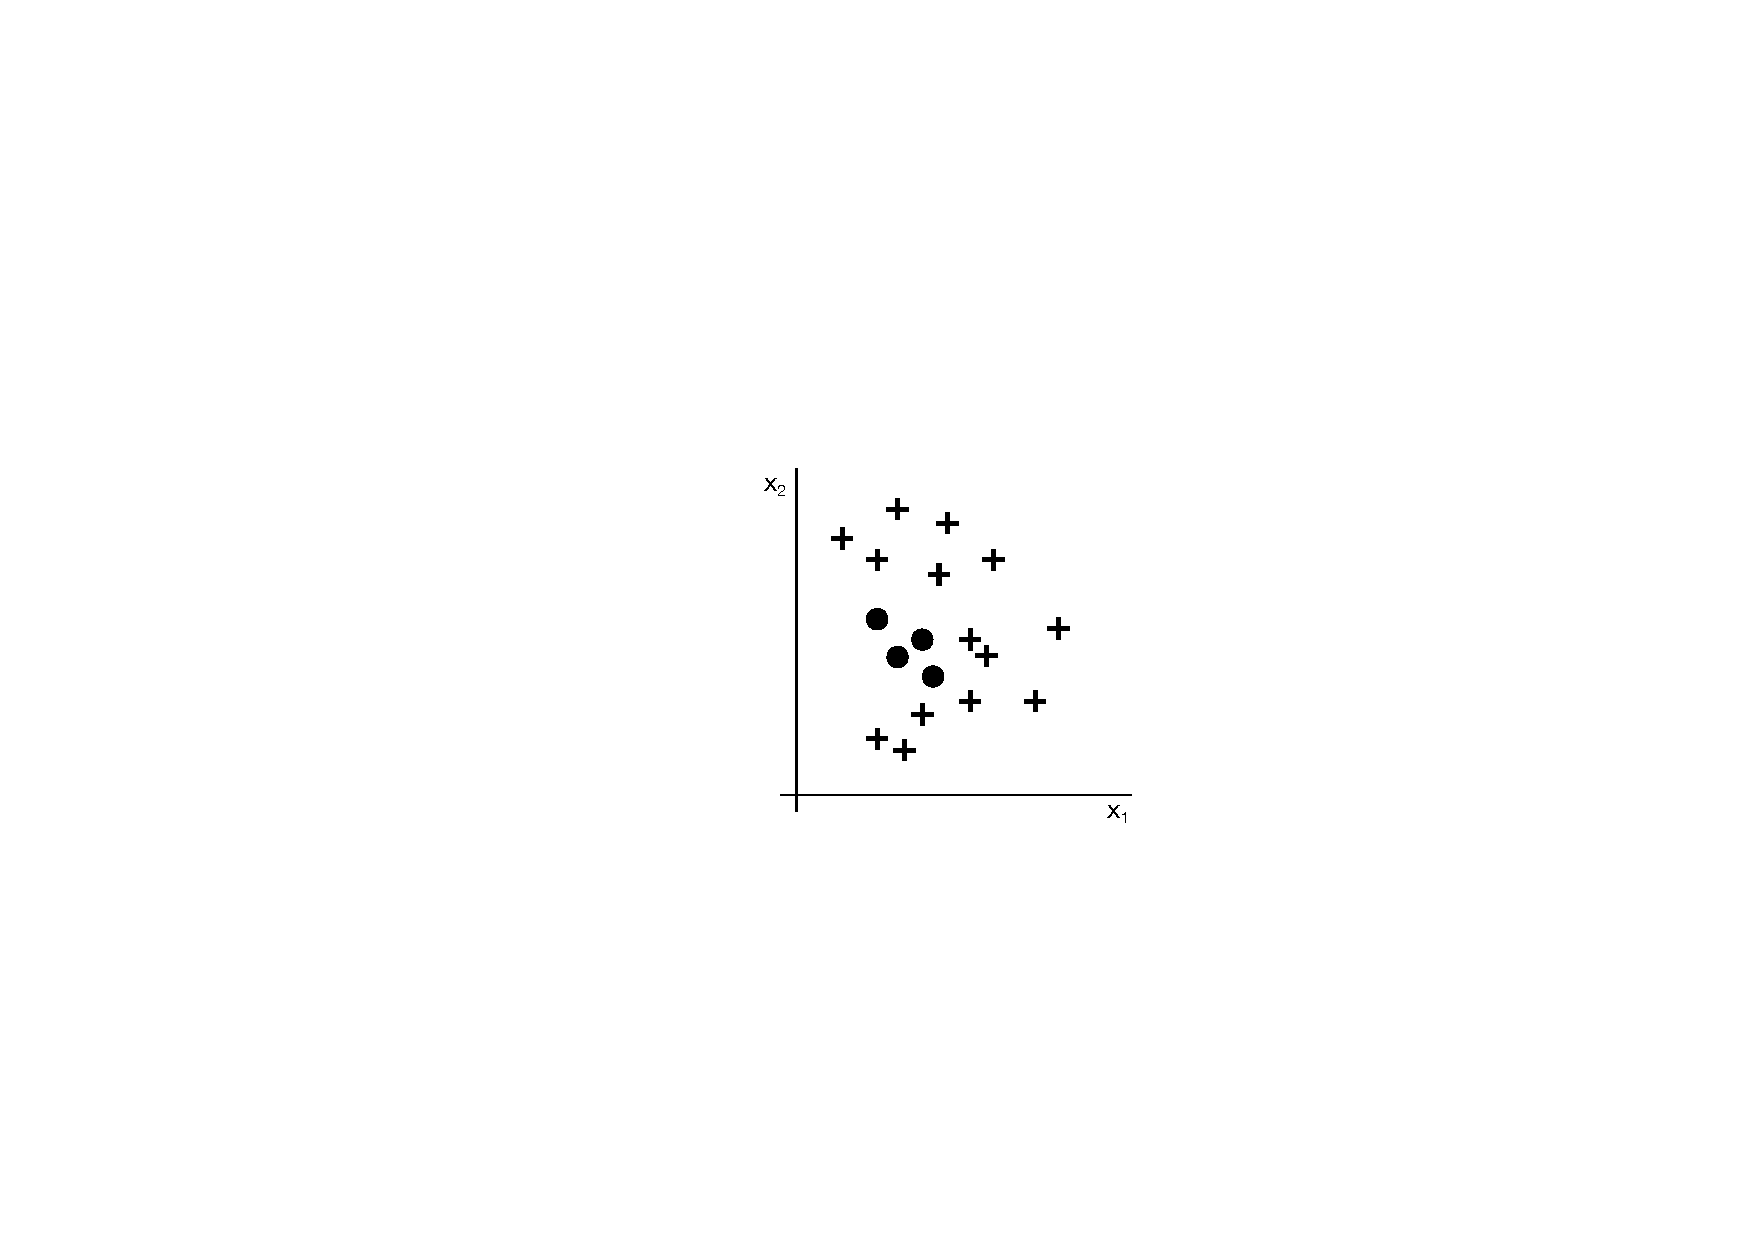
\includegraphics[width=0.3\linewidth]{figures/ann-hard-concept.pdf}
}
\caption{An example of a hard classification concept, where the classifier would need to recognize the interaction between two features, $x_1$ and $x_2$. Concepts like these are especially hard to model in the presence of many other features, which can be to a degree related to the class.}
\label{fig:hard-concept}
\end{figure}


A possible alternative to exhaustive search of feature interactions are models that incorporate feature interaction, and that can possibly model any kind of interaction between any of the features. The problem we are facing is of course the data. Such models need substantial, if not huge amount of data for training to avoid overfitting. But if data is available -- and sometimes it is -- then we better define the model that we can use in such cases. Notice that we are moving into direction where such models may be hard to explain, but this also is an issue we will deal with later, in our next chapter.


\section{Motivation from biology}

We start with disclaimer: artificial neural networks are very simplistic model of a brain, or any biological neural network. Biology is by orders of magnitude more complex: an axon, that is considered in artificial networks as a wire, has been studies in numerous projects and its structure and physiology has been reported in books of thousands of pages. With this warning, though, consider a realistic model of a neural cell in Fig.~\ref{fig:neural-cell}. Neural cell emits electric signals through the axon, but only when the potential in the cell body reaches a certain level, called {\em action potential}. The electrical potential of the body is a sum of potentials in the dendrites, and and this in turn depend on potential evoked from connected cells. Connections are established through synapses, which chemically transmit the electrical signal from the axon tips (inputs) to the dendrites. Neural cells thus, in a very simplified way, sum up the input signals and fire when the sum reaches specific threshold, emitting the signal through the axon and establishing a network with connected cells.

\begin{figure}
\centering{
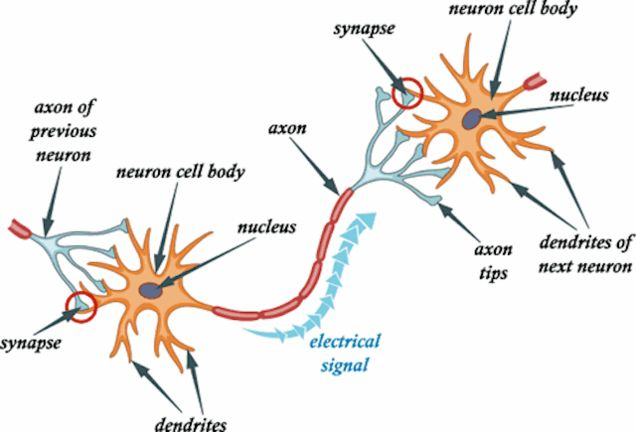
\includegraphics[width=0.8\linewidth]{figures/ann-neural-cell.jpg}
}
\caption{The structure of a neural cell, showing means of communication between two connected cells.}
\label{fig:neural-cell}
\end{figure}


Human brain contains $8\times 10^{10}$ neurons, where, on average, each neuron is connected to $10.000$ other neurons. The resulting network is huge and contains $10^{15}$, that is, $1.000$ trillion connections. 

Synapses adapt, adjusting the quantity of required transmitters and available receptors, thus implementing one of the mechanisms for plasticity of the brain and learning. Synapses, on the other hand, implement chemical transmission of the signals and are thus slow, but they are many and function in parallel.

The brain is modular. Different regions perform different functions. Experimentally this was observed in patients where local damages had specific effects. But the plasticity was observed as well: regions of brains can take over a specific function after the brain region originally carrying out this function was damaged. Damage in one region can therefore be alleviated through specialization of another region.

The idea of the network of neurons, neurons summing up the input signals, adaptivity of synapses which can weight the input, and a activation function implemented by a body of a neural cell are all concepts that are modeled by artificial neural networks. Brain plasticity and redundancy are modeled as well, and specifically addressed in larger, deeper neural networks.

\section{Idealized neuron}

Idealized neuron is a model of a neuronal cell with complicated details removed (Fig.~\ref{fig:idealized-neuron}). It performs simple mathematics, resorts to basic principles, and is wrong since the communication is not binary. The simplest model sums-up the inputs through a weighted sum, where $w_i$ is a weight for $i$-th input:
\begin{equation}
z = b + \sum_i x_i w_i,
\end{equation}
and the output of the {\em linear neuron} is
\begin{equation}
\hat{y} = z
\end{equation}

\begin{figure}
\centering{
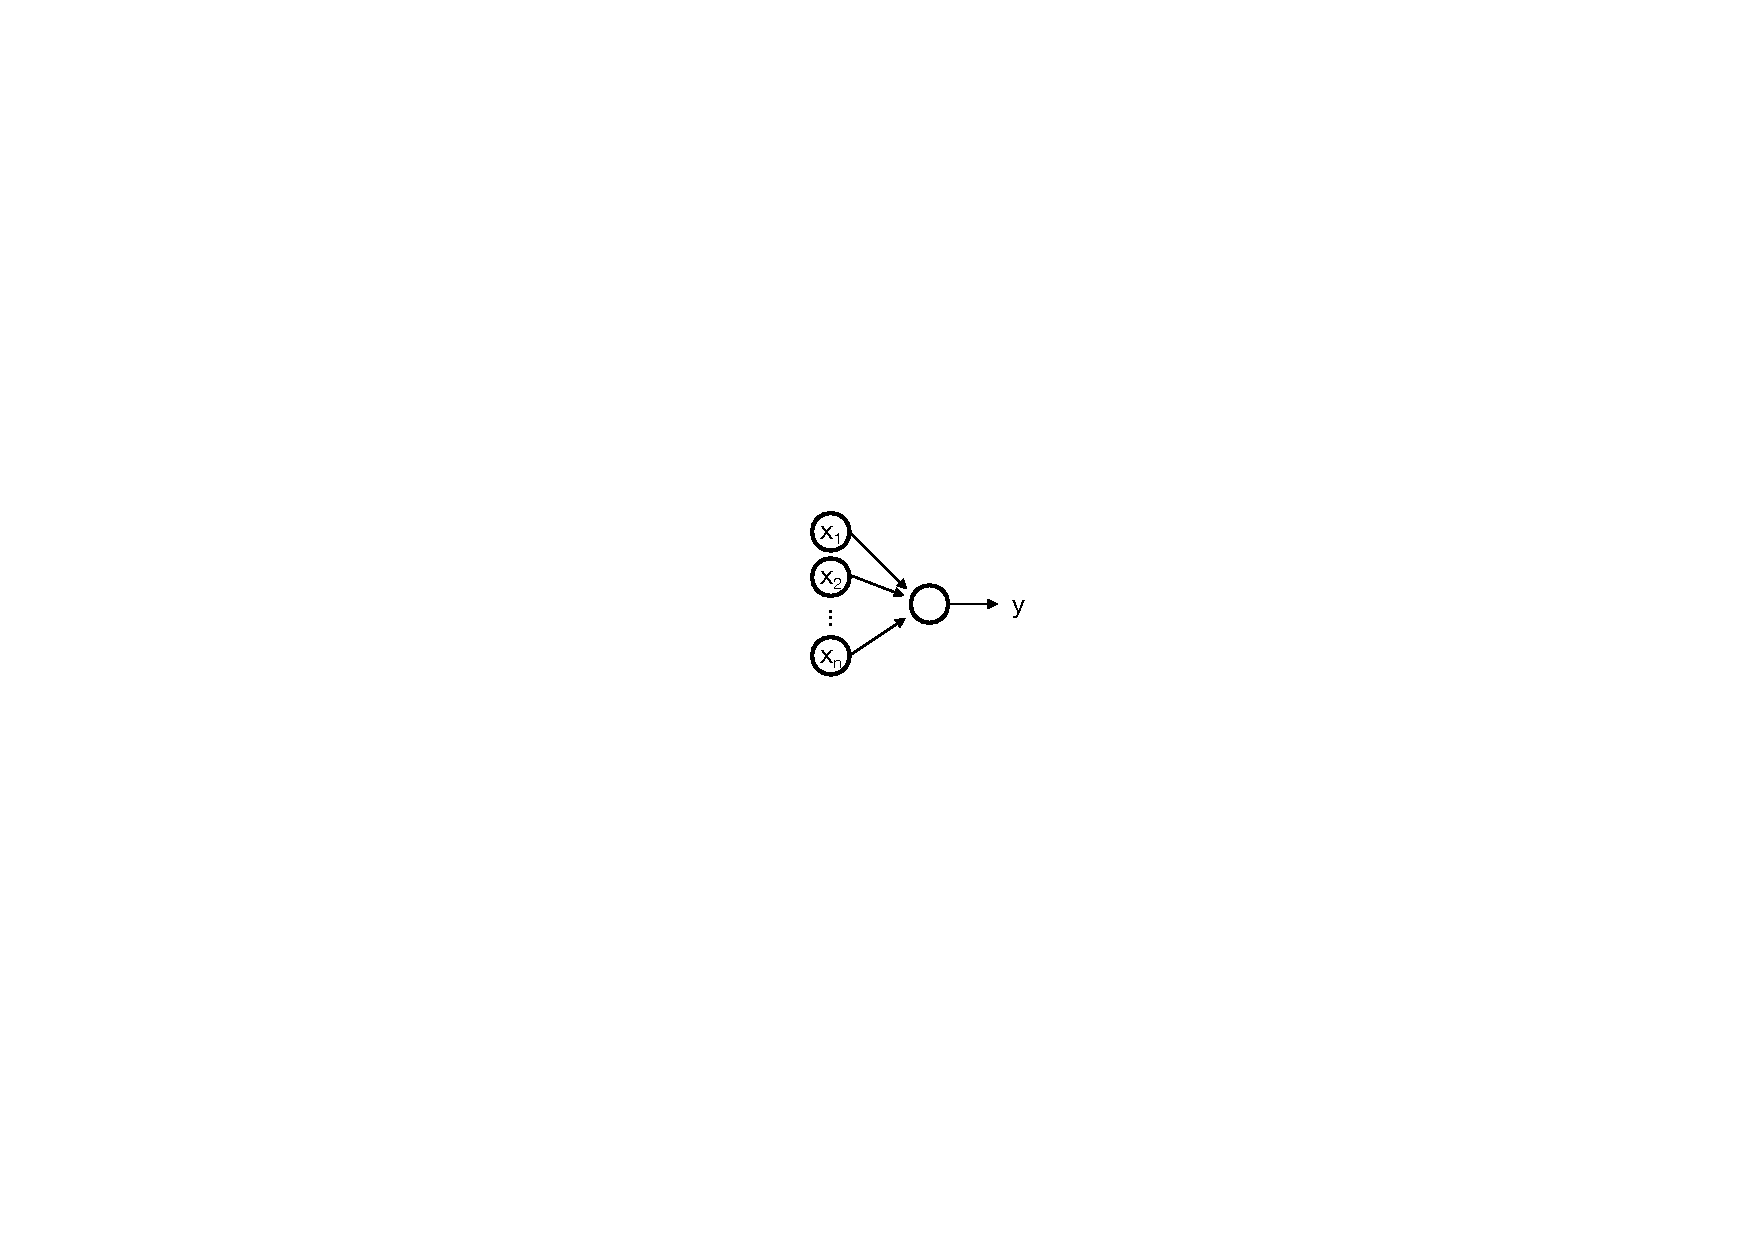
\includegraphics[width=0.3\linewidth]{figures/idealized-neuron.pdf}
}
\caption{An idealized neuron with $x_i$ representing its inputs and $y$ an output variable.}
\label{fig:idealized-neuron}
\end{figure}

Other types of neurons incorporate other {\em activation functions}, that is, functions that take a weighted sum of the inputs to compute the output of a neuron. Popular examples include {\em binary threshold neuron},
\begin{equation}
\hat{y} = 
\begin{cases}
1 & \text{if } z\geq 0 \\
0 & \text{else}
\end{cases}
\end{equation}
{\em rectified linear neuron}, or RELU,
\begin{equation}
\hat{y} = 
\begin{cases}
z & \text{if } z\geq 0 \\
0 & \text{else}
\end{cases}
\end{equation}
and {\em sigmoid neurons},
\begin{equation}
\hat{y}={1\over 1+e^{-z}}
\end{equation}
Notice that a sigmoid neuron looks very much like one of the classification models we have already studied. Which one, and what are the differences, if any?

\section{Perceptrons}

Training with a single linear neuron, that is, a neuron implementing $z=w^\tr x$ and a related classifier, 
\begin{equation}
\hat{y} = h(z) =
\begin{cases}
1 & \text{if } z\geq 0 \\
-1 & \text{else}
\end{cases}
\end{equation}
was popular in 1960s under the name perceptron. The perceptrons (Fig.~\ref{fig:perceptron-learning}, algorithm in Table~\ref{t:perceptron}) were proposed by Frank Rosenblatt, one of the pioneers of artificial intelligence, and were wrongly presented as a very powerful tool. In really, learning with perceptrons was very weak, could not handle noise, but is still historically interesting. 

\begin{table}[htbp]
\caption{Perceptron's learning procedure}
\begin{tabbing}
xxxx \= xxxx \= xxxx \= xxxx \kill
initialize $w$ \\
{\bf repeat} \\
\> choose $(x, y)$ from the training set \\
\> {\bf if} $h(z) \neq y$ \\
\> \> {\bf if} $h(z)=-1$ \\
\> \> \> $w\leftarrow w+x$ \\
\> \> {\bf else} \\
\> \> \> $w\leftarrow w-x$ \\
\end{tabbing}
\label{t:perceptron}
\end{table}

\begin{figure}[htbp]
\centering{
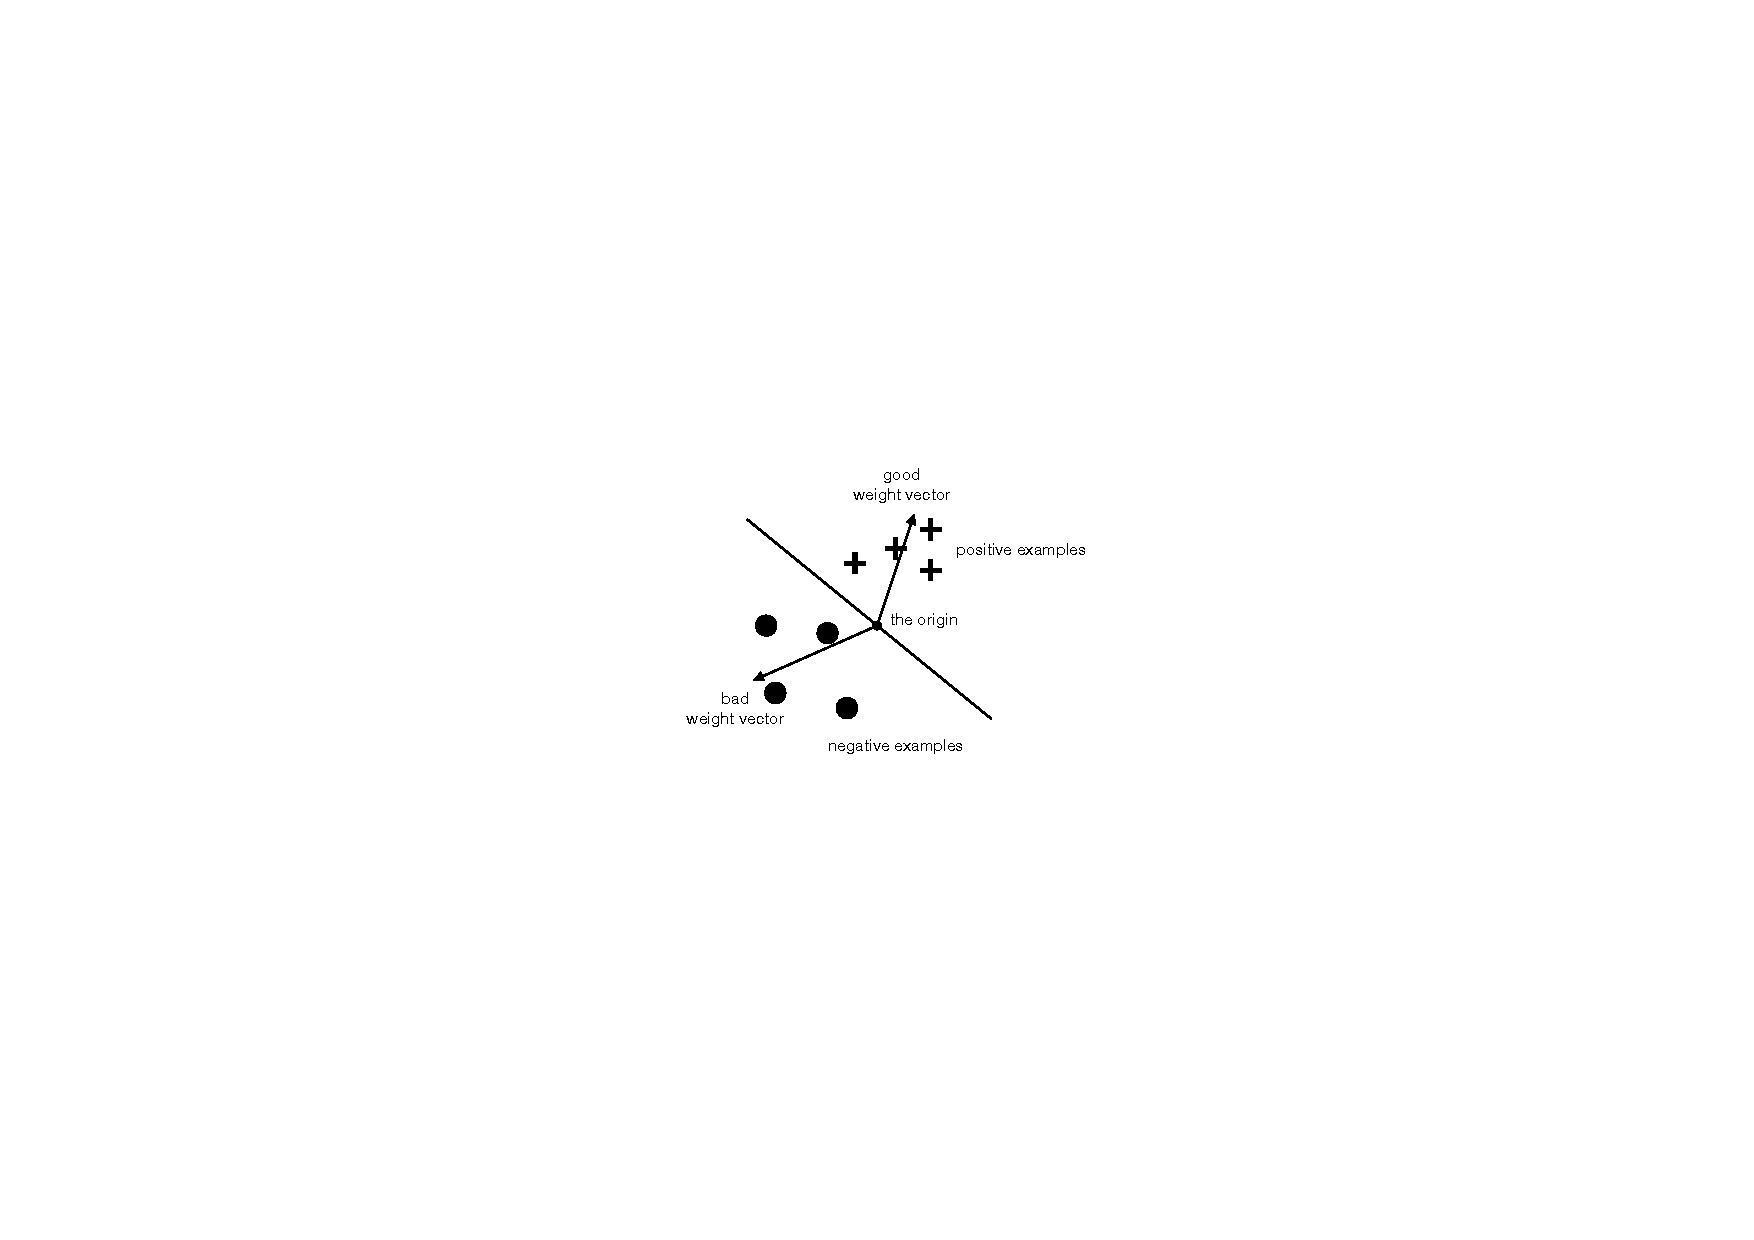
\includegraphics[width=0.3\linewidth]{figures/perceptron-learning.pdf}
}
\caption{Several concepts in perceptron learning.}
\label{fig:perceptron-learning}
\end{figure}

Notice that the perceptron training (Table~\ref{t:perceptron}) actually implements a stochastic gradient descent with a batch size of one and a learning rate of one. The training would succeed in cases where the classes are linearly separable, but fail otherwise. In linearly separable cases there would be infinitely many solutions where perceptron training would converge to a particular one. The process would fail under any interaction between input variables, where a typical example would be that of XOR. Obviously, there, we would need hierarchy of concepts and a nested perceptrons to model interactions.

\section{Artificial neural networks}

Artificial neural network is a network of artificial neurons. Output of one neuron is fed into inputs of a set of neurons. While there is no limitation on the structure of the network, the typical network starts with a layer of input features, continues with a layer of neurons, and then with the next layers, where each layer is fully connected. That is, a neuron at layer $L$ receives inputs from all neuron at previous level, level $L-1$. The last layer is special, and set according to the problem at hand. For instance, for regression, the last layer may include only one neuron, whose activation models variable $y$. For classification, the last layer may have as many neurons as there are class values, where each activation reports on a class probability. We refer to all layers between an input layer and an output layer as {\em hidden} layers.

Just like with other machine learning techniques, we have to set a cost function, and define a procedure to optimize the weights for each of the neuron accordingly. This procedure is known as {\em back-propagation}, and actually implements a gradient descent. We develop the mathematics for it in the next section.

\section{Back-propagation algorithm}

We start with some conventions. We assume that all units of the neural network can take value between 0 and 1. We refer to this value as {\em activation} and will denote it with $a$. In the previous text, when introducing a single neuron, we have denoted it with $\hat{y}$, which we will now reserve for the output of the entire network. We will also assume that the output of the neural network corresponds either to the value of regression problem, or to class probabilities, where of form of softmax regression is used to guarantee that the class probabilities sum to one.

To introduce the notation, consider a simple neural network with one input feature $x$ and one output $\hat{y}$, and one neuron in each of the two hidden layers (Fig.~\ref{fig:simple-network}).

\begin{figure}[htbp]
\centering{
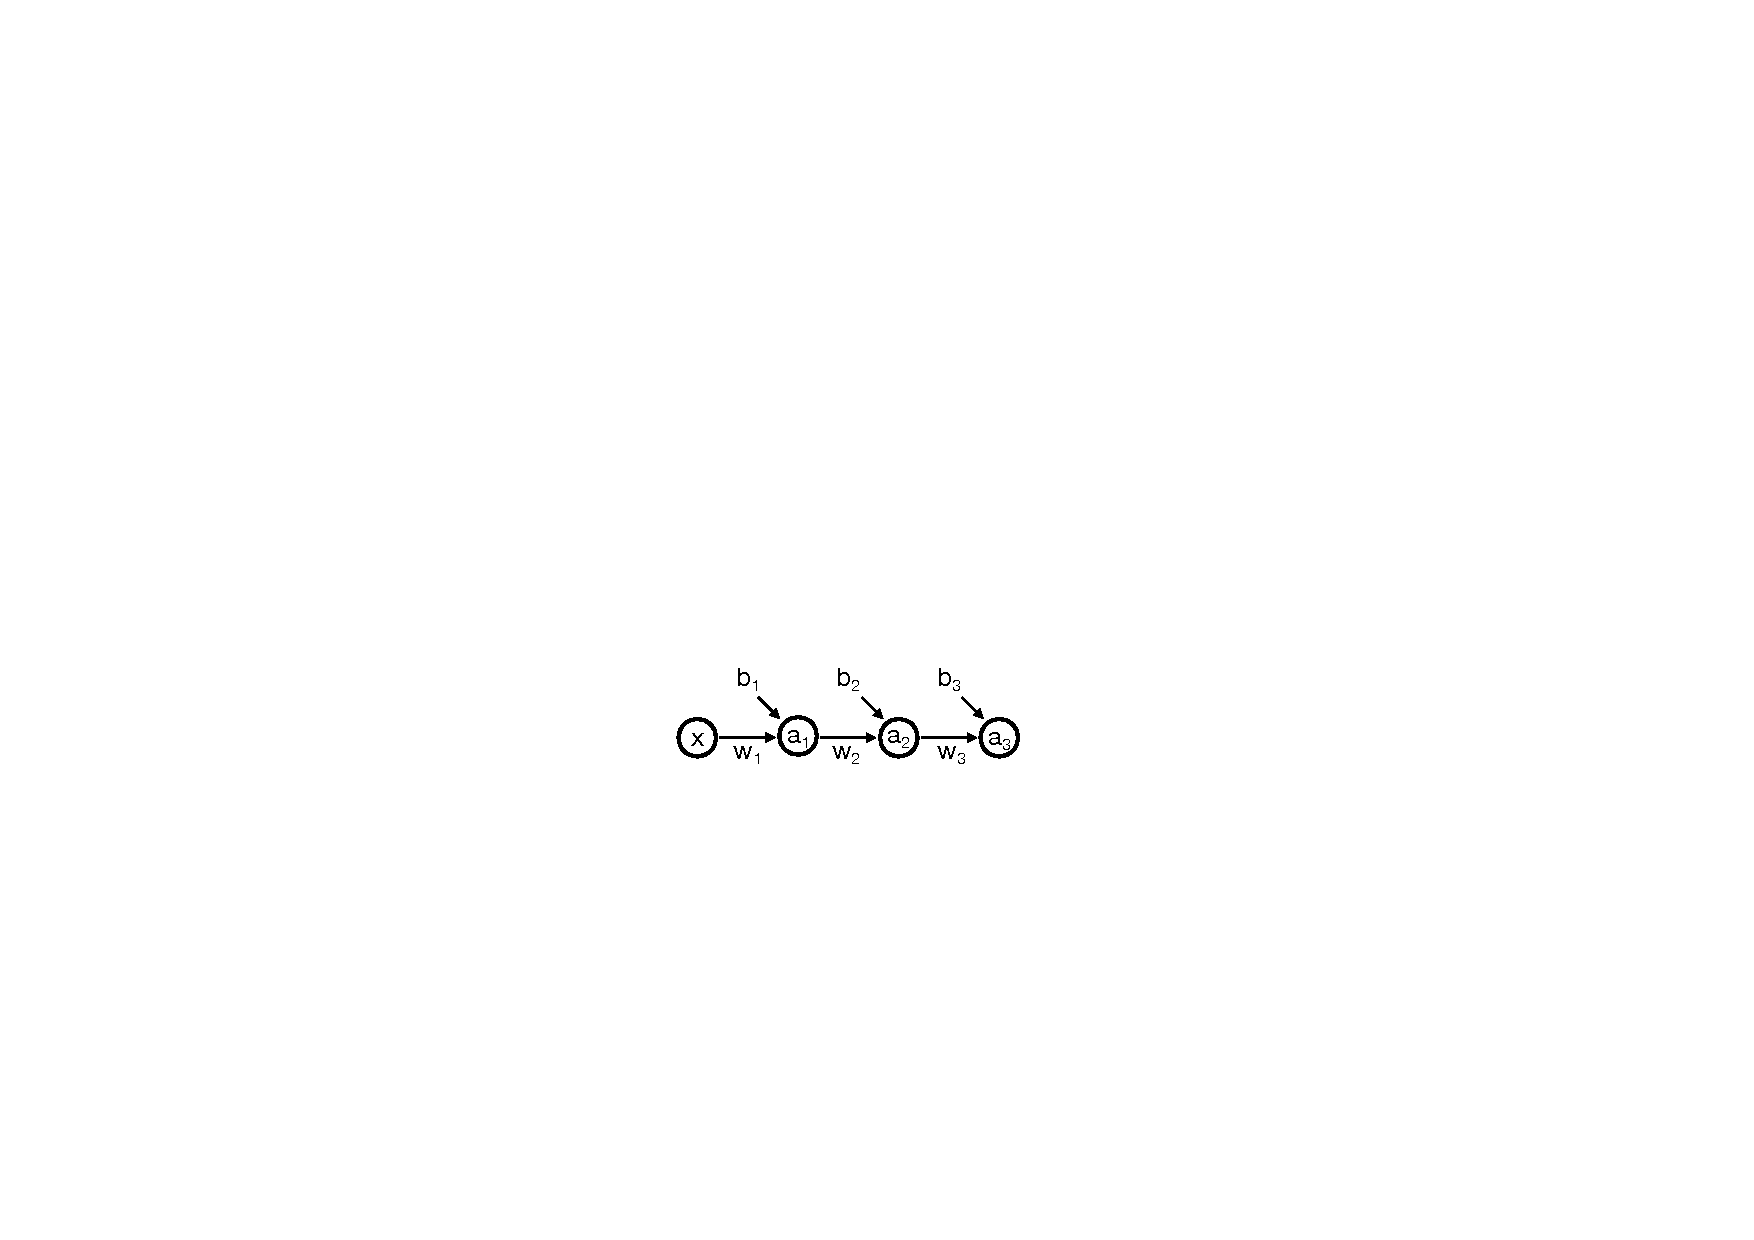
\includegraphics[width=0.5\linewidth]{figures/simple-network.pdf}
}
\caption{An example of a network with a single input and output and one neuron per layer.}
\label{fig:simple-network}
\end{figure}

Let us, for simplicity, assume we are dealing with only one example in the training set, and define a cost function as a squared error:
\begin{equation}
J(w_1, b_1, \ldots, w_3, b_3)=(a_3-y)^2
\end{equation}
Until now, we have used the indices to denote the weights $w$, the offsets $b$ and activation at each layer. Later, when dealing with more than one neuron at each layer, a notation which denotes the layer number will come handy. Apart from the layer with the input value, our simple network from Fig.~\ref{fig:simple-network} has three layers, $L=3$. The activation $a_3$ belongs to the third layer and we will alternatively denote it with $a^{(L)}$. Similarly, $a^{(L-1)}$ will denote $a_2$. Same goes with other parameters and activation values. We can thus write that the weighted sum of inputs for neuron at layer $L$ is equal to
\begin{equation}
z^{(L)}=w^{(L)} a^{(L-1)}+b^{(L)},
\end{equation}
the activation of that neuron is
\begin{equation}
a^{(L)}=\sigma(z^{(L)}),
\end{equation}
and the cost function
\begin{equation}
J(w_1, b_1, \ldots, w_3, b_3)=(a^{(L)}-y)^2
\end{equation}
While we can use any activation function here, we will sigmoid activation function for convenience.

To implement gradient descent, we need to find how does a cost function $J$ depend on the values of the parameters of the neural network. For instance, how does $J$ depend on the weight $w_3$, that is, the weight $w^{(L)}$? We can use a chain rule to compute the partial derivate, and while doing so, it helps us to examine the dependencies as depicted in Fig.~\ref{fig:dependency-tree}:
\begin{align}
\pd{J}{w^{(L)}} & = \pd{z^{(L)}}{w^{(L)}} \times \pd{a^{(L)}}{z^{(L)}} \times \pd{J}{a^{(L)}}\\
& = a^{(L-1)} \times \sigma(z)(1-sigma(z)) \times 2(a^{(L)}-y).
\end{align}
We can interpret the terms in this equation as $a^{(L-1)}$ denoting the power (or the weight) of the precious layer, $\sigma(z)(1-sigma(z))$ denoting a derivative of an activation function, and term $2(a^{(L)})-y)$ as the error of the prediction.

\begin{figure}[htbp]
\centering{
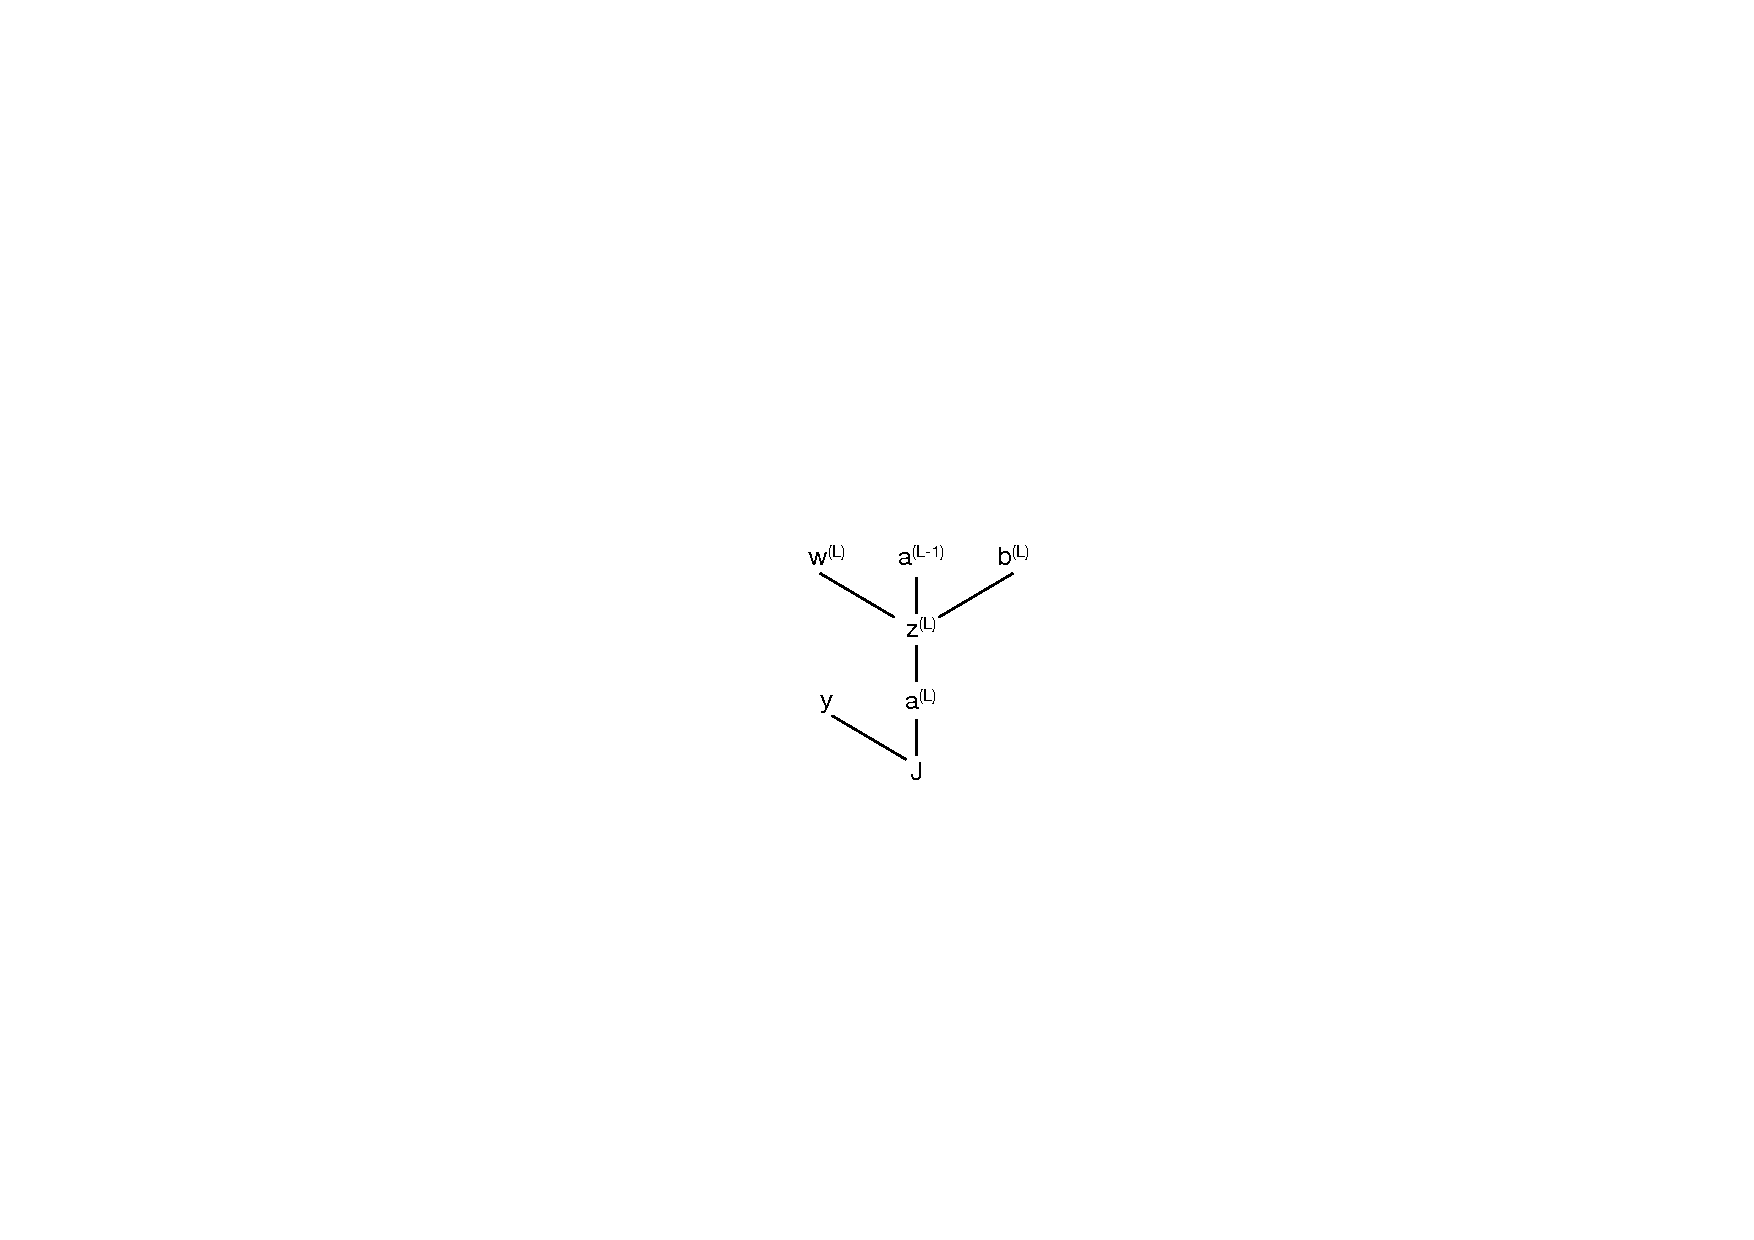
\includegraphics[width=0.3\linewidth]{figures/ann-dependency-tree.pdf}
}
\caption{Dependency tree of the cost function $J$ on some of the parameters from the neural network from Fig.~\ref{fig:simple-network}.}
\label{fig:dependency-tree}
\end{figure}

Above we have assumed we are dealing with only one training example. To generalize the above assertions for a set of training instances, we first need to modify the definition of the cost function, which now becomes:
\begin{equation}
J = \sum_{j=0}^N\left(a_j^{(L)}-y_j\right)^2
\end{equation}
Notice that the only change when computing partial derivative of $J$ according to $w^{(L)}$ is in computation of third term, $\pd{J}{a^{(L)}}$, which now becomes a sum of partial derivates.

\begin{figure}[htbp]
\centering{
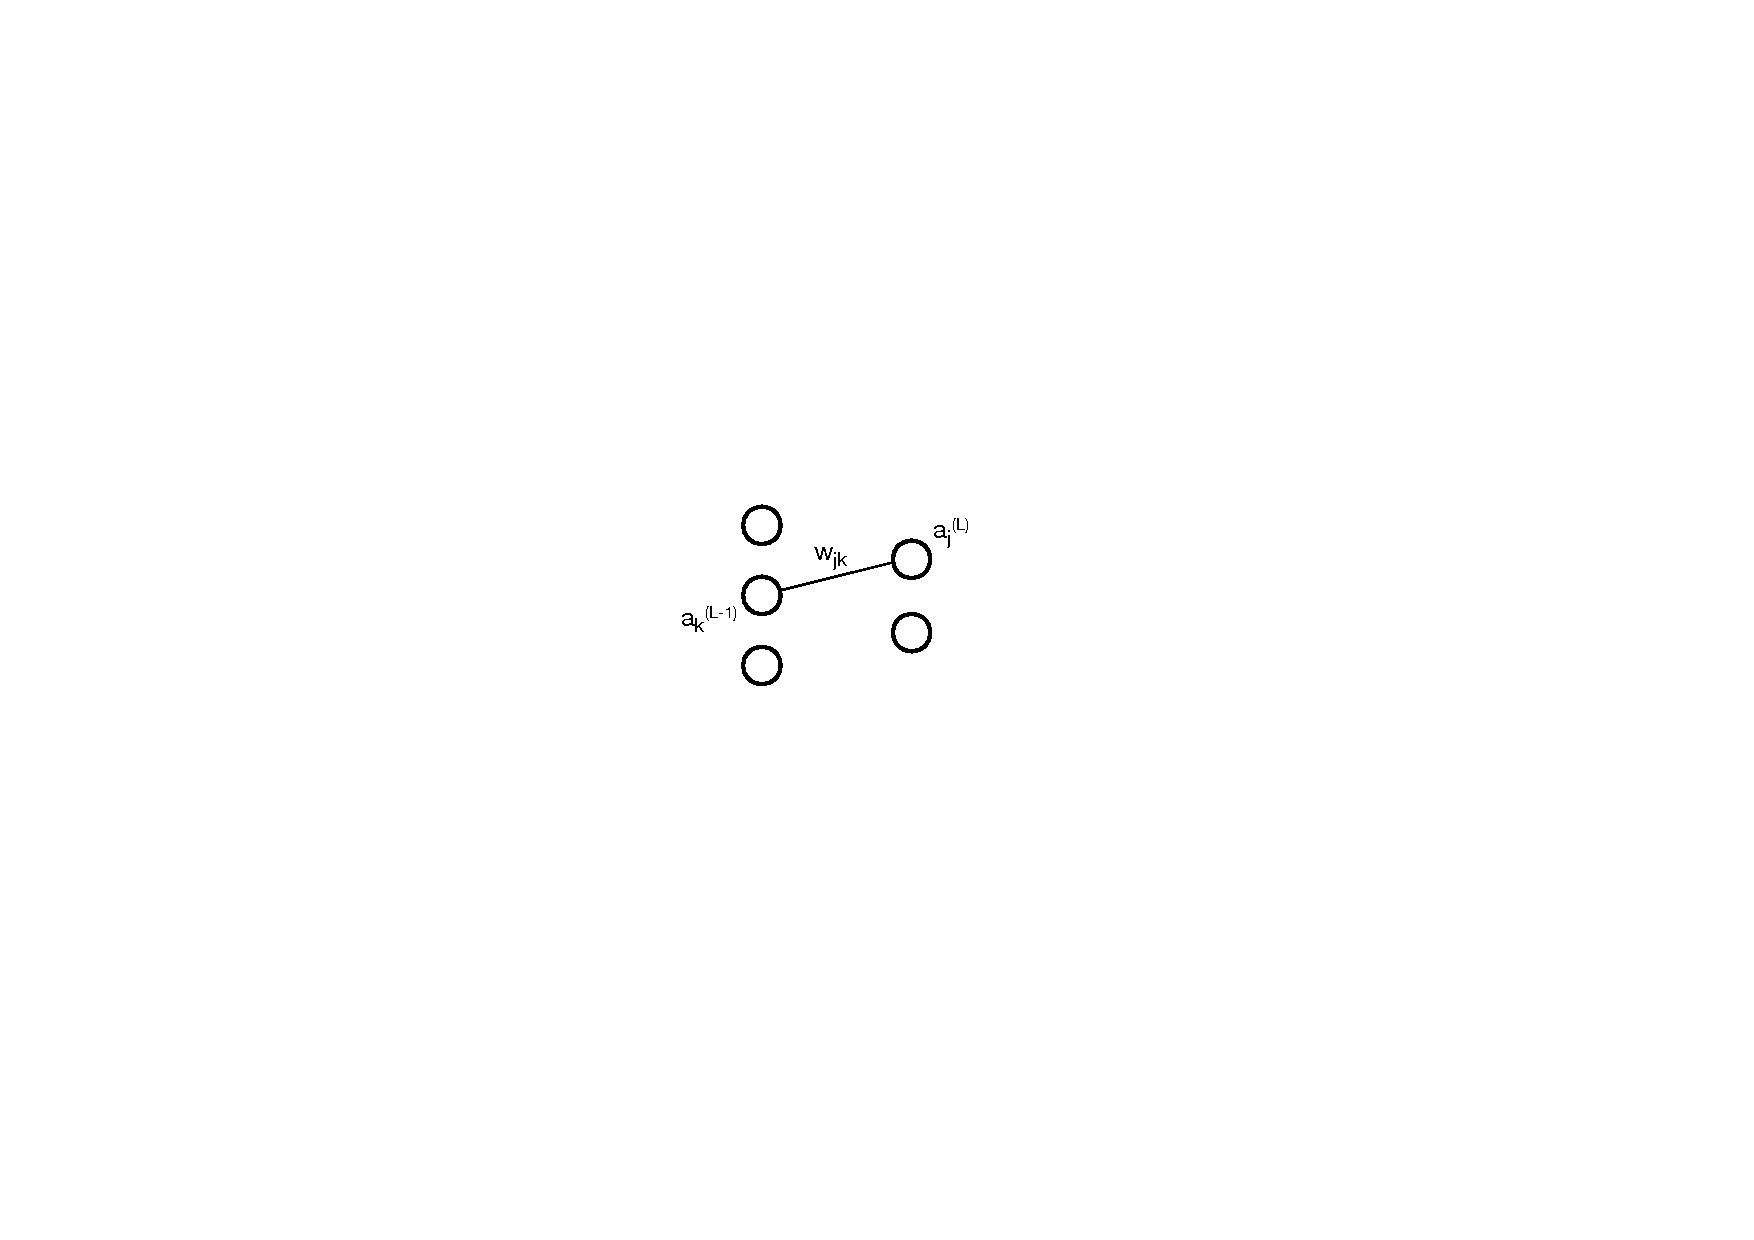
\includegraphics[width=0.3\linewidth]{figures/network-fragment.pdf}
}
\caption{A fragment of a neural network exposing the relation between activation of the $k$-th neuron in layer $(L-1)$ and activation of a $j$-th neuron at layer $L$.}
\label{fig:network-fragment}
\end{figure}

Let us consider now a more general type of network, with a number of neurons at each layer, and the number of neurons at the output layer. We again restrict the training set to only one data instance. Consider a fragment of a network from Fig.~\ref{fig:network-fragment}, which depicts the relation between activation of the $k$-th neuron in layer $(L-1)$ and $j$-th neuron at layer $L$. Notice that
\begin{align}
z_j^{(L)} & = \sum_i w_{ji}^{(L)} a_i^{(L-1)} + b_j^{(L)}, \\
a_j^{(L)} & = \sigma(z_j^{(L)}), \\
J & = \sum_j^{n_{L-1}}(a_j^{(L)}-y_j)^2.
\end{align}
We assume the indices run from 0, replace the intercepts $b$ for each $k$-th neuron with $w_{0k}$, and denote the number of neurons at layer $L$ with $n_L$. Notice also that the weights have now two indices. The weight $w_{jk}$ is a weight for a $j$-the neuron for the output of the $k$-th neuron from the previous layer. For a gradient descent, we again need to compute the change this weight invokes to the cost function,
\begin{equation}
\pd{J}{w_{jk}}=\sum_j\pd{z_j^{(L)}}{w_{jk}} \times \pd{a_j^{(L)}}{z_j^{(L)}} \times \pd{J}{a_j^{(L)}}
\end{equation}
The partial derivatives of the first two terms in the product are straightforward, and stem directly from the expression for $z_j^{(L)}$ and $a_j^{(L)}$. But the partial derivative in the last term is new, and we can break it down to
\begin{equation}
\pd{J}{a_k^{(L-1)}} = \sum_{j=0}^{n_L} \pd{z^{(L)}}{a_k^{(L-1)}} \times \pd{a_j^{(L)}}{z_j^{(L)}} \times \pd{J}{a_j^{(L)}}
\end{equation}
With these two expressions, we can now chain back through the network and compute the influence of every of the network's parameters, thus providing means for the gradient descent. The procedure is known under the name {\em back propagation}, which, intuitively:
\begin{itemize}
	\item converts discrepancy between output and and target into error derivative,
	\item computes the error derivatives in each hidden layer from error derivatives of the next layer,
	\item uses error derivative with respect to activations to get error derivative with respect to weights.
\end{itemize}

Let us express our derivations and back-propagation procedure in a matrix form. We will assume that the input data includes $m$ data instances and $n$ features, and will for convenience add a first column of $1$'s to the input data matrix, thus increasing its size to $m\times (n+1)$ and denoting this matrix with $\X'$. Let this matrix represent the activations of the neurons in the first, input layer:
\begin{equation}
\A^{(1)}=\X'
\end{equation}
Then we can write the equations for the second layer:
\begin{align}
\underset{m\times n_2}{\Z^{(2)}} & = \underset{m\times n_1}{\A}^{(1)} \underset{n_1\times n_2}{\W}^{(2)} \\
\underset{m\times n_2}{\A^{(2)}} & = \sigma\left( \underset{m\times n_2}{\Z^{(2)}} \right)
\end{align}
For the general $l$-th layer we can write:
\begin{equation}
A^{(l)} = \sigma\left(A^{(l-1)} W^{(l)}\right)
\end{equation}

We start with the last layer,
\begin{equation}
\pd{J}{\W^{(L)}} = \pd{\Z^{(L)}}{\W^{(l)}} \times \pd{\A^{(L)}}{\Z^{(L)}} \times \pd{J}{\A^{(L)}}
\end{equation}
where computing the first partial derivative is straightforward. Let us represent the product of the last two terms with $\mathrm{d}$:
\begin{align}
\underset{m\times n_L}{\mathrm{d}^{(L)}} & = \left(\A^{(L)}-\Y \right)  \odot \A^{(L)} \left( 1-\A^{(L)}\right) \\
\pd{J}{\W^{(L)}} & = {1\over m} \left(\A^{(L-1)} \right)^\tr \times \mathrm{d}^{(L)}
\end{align}
where with $\odot$ we denote element-wise product. In a similar way we compute the partial derivative $\pd{J}{\A^{(L-1)}}$ as a function of partial derivate of $\pd{J}{\A^{(L)}}$, and repeat the computation of the above two equations for lower levels of the network.

\section{Bag of tricks}

As with training of other classifiers and regression models, like linear and logistic regression, there are technique which can speed up and improve convergence of the training of neural networks. These, in brief, include:
\begin{itemize}
	\item To aim to prevent overfitting, we can use regularization, and include the sum of all the weights of the network in a cost function. This procedure was also known as a {\em weight decay}, where after the computation of each weight these well further scaled down by some factor, say $0.99$. Notice that if using sigmoid activation function, the small weights meant that we operate at the linear part of sigmoid at thus with regularization aim at derive close-to-linear model, thus simplifying it.
	\item Neural networks include many parameters, the problem we can alleviate through {\em weight sharing}. That is, neurons at some level would share some of the weights.
	\item Training of neural networks assumes large training data set. We can use all of the data instances from the training data, but for large data sets use {\em mini-batch} gradient descent with adaptive learning rate and use of momentum in the optimization.
	\item To further avoid overfitting, we can use {\em dropout}, where we randomly drop neurons along with their connections from the neural network during the training. Dropout prevents neurons from co-adapting. During training, dropout samples form an exponential number of different ``thinned'' networks, thus also, in some way, introduce ensembling.
\end{itemize}

These and other tricks and their details go beyond our discussion in this chapter. They are all implemented in today standard packages for neural network training. While one of the homeworks of this course will be on neural network implementation, this, and the derivation of related equations and their implementation would almost certainly be a once-in-a-lifetime attempt useful only for educational reasons.

\printbibliography[heading=subbibliography]
\end{refsection}
